\documentclass[12pt]{article}

% packages
\usepackage{kantlipsum}
\usepackage[margin=1in]{geometry}
\usepackage[labelfont=it]{caption}
\usepackage[table]{xcolor}
\usepackage{subcaption,framed,colortbl,multirow,multicol}
\usepackage{amsmath,amsthm,amssymb,wasysym,mathrsfs,mathtools}
\usepackage{tikz,graphicx,pgf,pgfplots}
\usetikzlibrary{arrows, angles, quotes, decorations.pathreplacing, math, patterns, calc}
\pgfplotsset{compat=1.16}

% custom commands
\newcommand{\N}{\mathbb{N}}
\newcommand{\Z}{\mathbb{Z}}
\newcommand{\I}{\mathbb{I}}
\newcommand{\R}{\mathbb{R}}
\newcommand{\Q}{\mathbb{Q}}
\newcommand{\C}{\mathbb{C}}
\newcommand{\p}{^{\prime}}
\newcommand{\powerset}{\raisebox{.15\baselineskip}{\Large\ensuremath{\wp}}}
\DeclarePairedDelimiter{\ceil}{\lceil}{\rceil}
\DeclarePairedDelimiter{\floor}{\lfloor}{\rfloor}

\newcommand{\exercise}[2]{\section*{Exercise #1}\framebox{\begin{minipage}{0.969\textwidth}#2\end{minipage}}\par\vspace{1em}}
\newcommand{\problem}[2]{\section*{Problem #1}\framebox{\begin{minipage}{0.969\textwidth}#2\end{minipage}}\par\vspace{1em}}

 
\begin{document}
 
\title{Assignment 2\\
    \large MATH CS 120FG Graph Theory I}
\author{Harry Coleman}
\date{January 23, 2020}
\maketitle


\exercise{2}{
    Prove that the average degree of any tree $T$ is less than 2.
}

Suppose $T$ is a tree with $n\geq1$ vertices. We know that $T$ must have $n-1$ edges. By the handshaking lemma, the total degree of $T$ is $2(n-1)$. Dividing by the number of vertices, we find the average degree of $T$ to be
\[\frac{2(n-1)}{n} = 2-\frac{1}{n} < 2.\]


\exercise{3}{
    Let $T$ be a tree on $n > 1$ vertices in which all vertices have degree at most 3. Let $d_3(T)$ denote the number of vertices of degree 3 in such a tree $T$. Prove that
    \[d_3(T) \leq \floor*{\frac{n-2}{2}}.\]
}

Consider the degree sequence of $T$,
\[(\underbrace{3,\dots,3}_{d_3(T)}, \underbrace{2,\dots,2}_{d_2(T)}, \underbrace{1,\dots,1}_{d_1(T)}),\]
where there are $d_i(T)$ vertices with degree $i$. The sum of all $d_i(T)$ gives us the number of vertices $n$ and the sum of all $i\cdot d_i(T)$ gives us the total degree of $T$, which is $2(n-1)$ by the handshaking lemma. So,
\begin{alignat*}{4}
    3d_3(T) &+& 2d_2(T) &+& 1d_1(T) &= 2(n-1), \\
    d_3(T) &+& d_2(T) &+& d_1(T) &= n.
\end{alignat*}
Subtracting the two equations, we find
\begin{alignat*}{4}
    2d_3(T) &+& 1d_2(T) &+& 0d_1(T) &= 2n-2 - n, \\
    2d_3(T) &+& d_2(T) &&  &= n - 2.
\end{alignat*}
Since $d_2(T)$ is some nonnegative number,
\begin{align*}
    2d_3(T) &\leq 2d_3(T) + d_2(T) = n-2, \\
    d_3(T) &\leq \frac{n-2}{2}, \\
    \floor*{d_3(T)} &\leq \floor*{\frac{n-2}{2}}, \\
    d_3(T) &\leq \floor*{\frac{n-2}{2}}.
\end{align*}



\exercise{4}{
    Generalize the previous question by, for a given $k \geq 3$, finding an upper bound for $d_k(T)$ where $T$ is a tree in which every vertex has degree at most $k$.
}

Let $T$ be a tree with $n$ vertices. Again taking $d_i(T)$ to be the number of vertices in $T$ with degree $i$, we find that
\[\sum_{i=1}^k d_i(T) = n,\]
and by the handshaking lemma,
\[\sum_{i=1}^k i\cdot d_i(T) = 2(n-1).\]
Taking the difference, we obtain
\begin{align*}
    \sum_{i=1}^k i\cdot d_i(T) - \sum_{i=1}^k d_i(T) &= n-2, \\
    \sum_{i=1}^k [i\cdot d_i(T) - d_i(T)] &= n-2, \\
    \sum_{i=1}^k [(i-1)\cdot d_i(T)] &= n-2, \\
    (k-1)d_k(T) + \sum_{i=1}^{k-1} [(i-1)\cdot d_i(T)] &= n-2.
\end{align*}
Since $\sum_{i=1}^{k-1} [(i-1)\cdot d_i(T)]$ is some nonnegative number, we can perform the same series of steps from exercise 3 to find
\[(k-1)d_k(T) \leq (k-1)d_k(T) + \sum_{i=1}^{k-1} [(i-1)\cdot d_i(T)] = n-2,\]
\[d_k(T) \leq \floor*{\frac{n-2}{k-1}}.\]


\exercise{5}{
    Apply Kruskal’s algorithm to the graph in Figure 1 to find a minimum spanning tree (list out the edges in each step of the algorithm and draw the final MST.)
}

At each step, we will select the cheapest edge, keeping a forest. The edge chosen $(u,v)$ and its cost is noted at each step.
\begin{enumerate}
    \item (2,4): -2
    \item (2,5): -2
    \item (3,4): 0
    \item (5,6): 0
    \item (1,10): 1
    \item (1,9): 2
    \item (1,11): 3
    \item (8,9): 3
    \item (1,7): 5
    \item (3,11): 6
\end{enumerate}

These edges give us the following spanning tree:

\begin{center}
    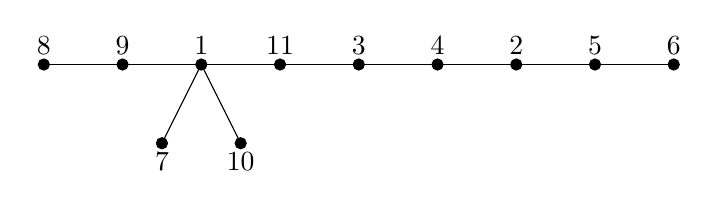
\begin{tikzpicture}
        \draw[fill=black] (0,0) circle (2pt) node[anchor=south]{8};
        \draw[fill=black] (1,0) circle (2pt) node[anchor=south]{9};
        \draw[fill=black] (2,0) circle (2pt) node[anchor=south]{1};
        \draw[fill=black] (3,0) circle (2pt) node[anchor=south]{11};
        \draw[fill=black] (4,0) circle (2pt) node[anchor=south]{3};
        \draw[fill=black] (5,0) circle (2pt) node[anchor=south]{4};
        \draw[fill=black] (6,0) circle (2pt) node[anchor=south]{2};
        \draw[fill=black] (7,0) circle (2pt) node[anchor=south]{5};
        \draw[fill=black] (8,0) circle (2pt) node[anchor=south]{6};
        \draw[fill=black] (1.5,-1) circle (2pt) node[anchor=north]{7};
        \draw[fill=black] (2.5,-1) circle (2pt) node[anchor=north]{10};
        
        \draw[] (0,0)--(8,0);
        \draw[] (2.5,-1)--(2,0)--(1.5,-1);
        
    \end{tikzpicture}
\end{center}


\newpage
\exercise{6}{
    Draw the trees corresponding to the Pr{\"u}fer codes (5, 2, 1, 1, 8, 2) and (1, 2, 3, 3, 3, 2, 1).
}

\begin{multicols}{2}
\begin{align*}
    \text{code: } & (5, 2, 1, 1, 8, 2) \\
    \text{vertices: } & (1, 2, 3, 4, 5, 6, 7, 8)
\end{align*}
\begin{center}
    \begin{tikzpicture}
        \draw[fill=black] (0,0) circle (2pt) node[anchor=south]{3};
        \draw[fill=black] (1,0) circle (2pt) node[anchor=south]{5};
        \draw[fill=black] (2,0) circle (2pt) node[anchor=south]{1};
        \draw[fill=black] (3,0) circle (2pt) node[anchor=south]{8};
        \draw[fill=black] (4,0) circle (2pt) node[anchor=south]{2};
        \draw[fill=black] (5,0) circle (2pt) node[anchor=south]{4};
        \draw[fill=black] (2,-1) circle (2pt) node[anchor=north]{6};
        \draw[fill=black] (4,-1) circle (2pt) node[anchor=north]{7};
    \end{tikzpicture}
\end{center}

\begin{align*}
    \text{code: } & (\not5, 2, 1, 1, 8, 2) \\
    \text{vertices: } & (1, 2, \not3, 4, 5, 6, 7, 8)
\end{align*}
\begin{center}
    \begin{tikzpicture}
        \draw[fill=black] (0,0) circle (2pt) node[anchor=south]{3};
        \draw[fill=black] (1,0) circle (2pt) node[anchor=south]{5};
        \draw[fill=black] (2,0) circle (2pt) node[anchor=south]{1};
        \draw[fill=black] (3,0) circle (2pt) node[anchor=south]{8};
        \draw[fill=black] (4,0) circle (2pt) node[anchor=south]{2};
        \draw[fill=black] (5,0) circle (2pt) node[anchor=south]{4};
        \draw[fill=black] (2,-1) circle (2pt) node[anchor=north]{6};
        \draw[fill=black] (4,-1) circle (2pt) node[anchor=north]{7};
        
        \draw[] (0,0)--(1,0);
    \end{tikzpicture}
\end{center}

\begin{align*}
    \text{code: } & (\not5, \not2, 1, 1, 8, 2) \\
    \text{vertices: } & (1, 2, \not3, \not4, 5, 6, 7, 8)
\end{align*}
\begin{center}
    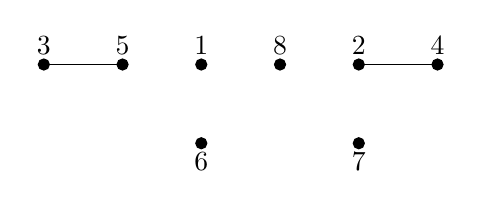
\begin{tikzpicture}
        \draw[fill=black] (0,0) circle (2pt) node[anchor=south]{3};
        \draw[fill=black] (1,0) circle (2pt) node[anchor=south]{5};
        \draw[fill=black] (2,0) circle (2pt) node[anchor=south]{1};
        \draw[fill=black] (3,0) circle (2pt) node[anchor=south]{8};
        \draw[fill=black] (4,0) circle (2pt) node[anchor=south]{2};
        \draw[fill=black] (5,0) circle (2pt) node[anchor=south]{4};
        \draw[fill=black] (2,-1) circle (2pt) node[anchor=north]{6};
        \draw[fill=black] (4,-1) circle (2pt) node[anchor=north]{7};
        
        \draw[] (0,0)--(1,0);
        \draw[] (4,0)--(5,0);
    \end{tikzpicture}
\end{center}

\begin{align*}
    \text{code: } & (\not5, \not2, \not1, 1, 8, 2) \\
    \text{vertices: } & (1, 2, \not3, \not4, \not5, 6, 7, 8)
\end{align*}
\begin{center}
    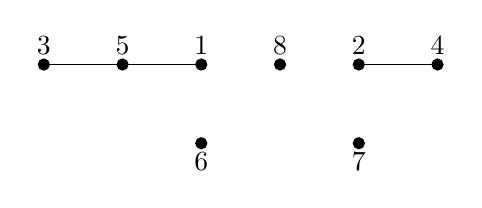
\begin{tikzpicture}
        \draw[fill=black] (0,0) circle (2pt) node[anchor=south]{3};
        \draw[fill=black] (1,0) circle (2pt) node[anchor=south]{5};
        \draw[fill=black] (2,0) circle (2pt) node[anchor=south]{1};
        \draw[fill=black] (3,0) circle (2pt) node[anchor=south]{8};
        \draw[fill=black] (4,0) circle (2pt) node[anchor=south]{2};
        \draw[fill=black] (5,0) circle (2pt) node[anchor=south]{4};
        \draw[fill=black] (2,-1) circle (2pt) node[anchor=north]{6};
        \draw[fill=black] (4,-1) circle (2pt) node[anchor=north]{7};
        
        \draw[] (0,0)--(1,0);
        \draw[] (4,0)--(5,0);
        \draw[] (1,0)--(2,0);
    \end{tikzpicture}
\end{center}

\begin{align*}
    \text{code: } & (\not5, \not2, \not1, \not1, 8, 2) \\
    \text{vertices: } & (1, 2, \not3, \not4, \not5, \not6, 7, 8)
\end{align*}
\begin{center}
    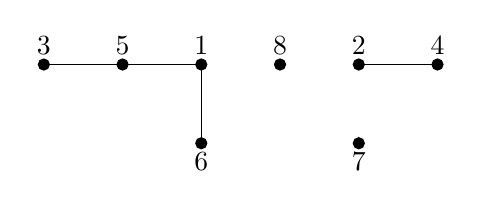
\begin{tikzpicture}
        \draw[fill=black] (0,0) circle (2pt) node[anchor=south]{3};
        \draw[fill=black] (1,0) circle (2pt) node[anchor=south]{5};
        \draw[fill=black] (2,0) circle (2pt) node[anchor=south]{1};
        \draw[fill=black] (3,0) circle (2pt) node[anchor=south]{8};
        \draw[fill=black] (4,0) circle (2pt) node[anchor=south]{2};
        \draw[fill=black] (5,0) circle (2pt) node[anchor=south]{4};
        \draw[fill=black] (2,-1) circle (2pt) node[anchor=north]{6};
        \draw[fill=black] (4,-1) circle (2pt) node[anchor=north]{7};
        
        \draw[] (0,0)--(1,0);
        \draw[] (4,0)--(5,0);
        \draw[] (1,0)--(2,0);
        \draw[] (2,0)--(2,-1);
    \end{tikzpicture}
\end{center}

\begin{align*}
    \text{code: } & (\not5, \not2, \not1, \not1, \not8, 2) \\
    \text{vertices: } & (\not1, 2, \not3, \not4, \not5, \not6, 7, 8)
\end{align*}
\begin{center}
    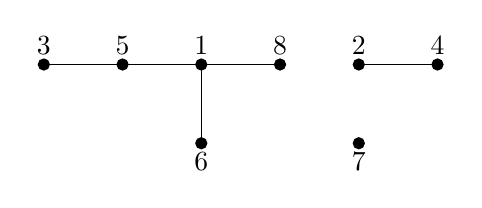
\begin{tikzpicture}
        \draw[fill=black] (0,0) circle (2pt) node[anchor=south]{3};
        \draw[fill=black] (1,0) circle (2pt) node[anchor=south]{5};
        \draw[fill=black] (2,0) circle (2pt) node[anchor=south]{1};
        \draw[fill=black] (3,0) circle (2pt) node[anchor=south]{8};
        \draw[fill=black] (4,0) circle (2pt) node[anchor=south]{2};
        \draw[fill=black] (5,0) circle (2pt) node[anchor=south]{4};
        \draw[fill=black] (2,-1) circle (2pt) node[anchor=north]{6};
        \draw[fill=black] (4,-1) circle (2pt) node[anchor=north]{7};
        
        \draw[] (0,0)--(1,0);
        \draw[] (4,0)--(5,0);
        \draw[] (1,0)--(2,0);
        \draw[] (2,0)--(2,-1);
        \draw[] (2,0)--(3,0);
    \end{tikzpicture}
\end{center}

\begin{align*}
    \text{code: } & (\not5, \not2, \not1, \not1, \not8, \not2) \\
    \text{vertices: } & (\not1, 2, \not3, \not4, \not5, \not6, \not7, 8)
\end{align*}
\begin{center}
    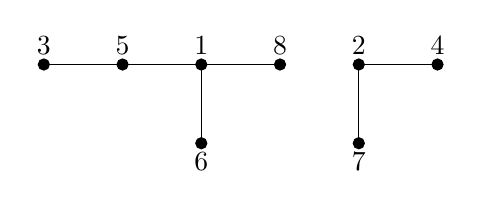
\begin{tikzpicture}
        \draw[fill=black] (0,0) circle (2pt) node[anchor=south]{3};
        \draw[fill=black] (1,0) circle (2pt) node[anchor=south]{5};
        \draw[fill=black] (2,0) circle (2pt) node[anchor=south]{1};
        \draw[fill=black] (3,0) circle (2pt) node[anchor=south]{8};
        \draw[fill=black] (4,0) circle (2pt) node[anchor=south]{2};
        \draw[fill=black] (5,0) circle (2pt) node[anchor=south]{4};
        \draw[fill=black] (2,-1) circle (2pt) node[anchor=north]{6};
        \draw[fill=black] (4,-1) circle (2pt) node[anchor=north]{7};
        
        \draw[] (0,0)--(1,0);
        \draw[] (4,0)--(5,0);
        \draw[] (1,0)--(2,0);
        \draw[] (2,0)--(2,-1);
        \draw[] (2,0)--(3,0);
        \draw[] (4,0)--(4,-1);
    \end{tikzpicture}
\end{center}

\begin{align*}
    \text{code: } & (\not5, \not2, \not1, \not1, \not8, \not2) \\
    \text{vertices: } & (\not1, \not2, \not3, \not4, \not5, \not6, \not7, \not8)
\end{align*}
\begin{center}
    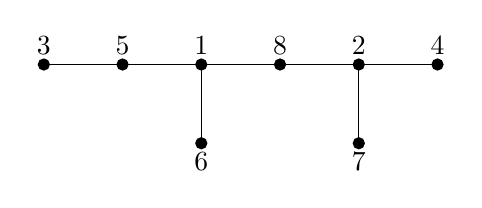
\begin{tikzpicture}
        \draw[fill=black] (0,0) circle (2pt) node[anchor=south]{3};
        \draw[fill=black] (1,0) circle (2pt) node[anchor=south]{5};
        \draw[fill=black] (2,0) circle (2pt) node[anchor=south]{1};
        \draw[fill=black] (3,0) circle (2pt) node[anchor=south]{8};
        \draw[fill=black] (4,0) circle (2pt) node[anchor=south]{2};
        \draw[fill=black] (5,0) circle (2pt) node[anchor=south]{4};
        \draw[fill=black] (2,-1) circle (2pt) node[anchor=north]{6};
        \draw[fill=black] (4,-1) circle (2pt) node[anchor=north]{7};
        
        \draw[] (0,0)--(1,0);
        \draw[] (4,0)--(5,0);
        \draw[] (1,0)--(2,0);
        \draw[] (2,0)--(2,-1);
        \draw[] (2,0)--(3,0);
        \draw[] (4,0)--(4,-1);
        \draw[] (3,0)--(4,0);
    \end{tikzpicture}
\end{center}

\end{multicols}

\begin{multicols}{2}
\begin{align*}
    \text{code: } & (1, 2, 3, 3, 3, 2, 1) \\
    \text{vertices: } & (1, 2, 3, 4, 5, 6, 7, 8, 9)
\end{align*}
\begin{center}
    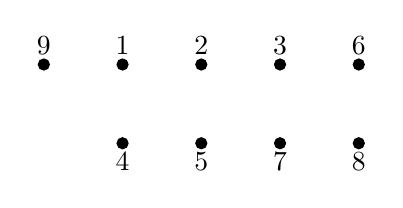
\begin{tikzpicture}
        \draw[fill=black] (0,0) circle (2pt) node[anchor=south]{9};
        \draw[fill=black] (1,0) circle (2pt) node[anchor=south]{1};
        \draw[fill=black] (2,0) circle (2pt) node[anchor=south]{2};
        \draw[fill=black] (3,0) circle (2pt) node[anchor=south]{3};
        \draw[fill=black] (4,0) circle (2pt) node[anchor=south]{6};
        \draw[fill=black] (1,-1) circle (2pt) node[anchor=north]{4};
        \draw[fill=black] (2,-1) circle (2pt) node[anchor=north]{5};
        \draw[fill=black] (3,-1) circle (2pt) node[anchor=north]{7};
        \draw[fill=black] (4,-1) circle (2pt) node[anchor=north]{8};
    \end{tikzpicture}
\end{center}

\begin{align*}
    \text{code: } & (\not1, 2, 3, 3, 3, 2, 1) \\
    \text{vertices: } & (1, 2, 3, \not4, 5, 6, 7, 8, 9)
\end{align*}
\begin{center}
    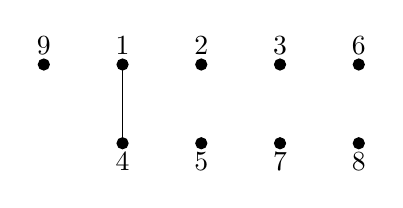
\begin{tikzpicture}
        \draw[fill=black] (0,0) circle (2pt) node[anchor=south]{9};
        \draw[fill=black] (1,0) circle (2pt) node[anchor=south]{1};
        \draw[fill=black] (2,0) circle (2pt) node[anchor=south]{2};
        \draw[fill=black] (3,0) circle (2pt) node[anchor=south]{3};
        \draw[fill=black] (4,0) circle (2pt) node[anchor=south]{6};
        \draw[fill=black] (1,-1) circle (2pt) node[anchor=north]{4};
        \draw[fill=black] (2,-1) circle (2pt) node[anchor=north]{5};
        \draw[fill=black] (3,-1) circle (2pt) node[anchor=north]{7};
        \draw[fill=black] (4,-1) circle (2pt) node[anchor=north]{8};
        
        \draw[] (1,0)--(1,-1);
    \end{tikzpicture}
\end{center}

\begin{align*}
    \text{code: } & (\not1, \not2, 3, 3, 3, 2, 1) \\
    \text{vertices: } & (1, 2, 3, \not4, \not5, 6, 7, 8, 9)
\end{align*}
\begin{center}
    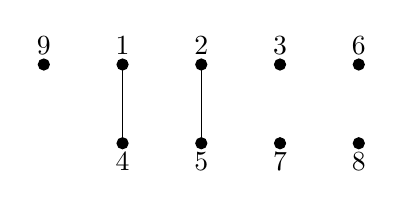
\begin{tikzpicture}
        \draw[fill=black] (0,0) circle (2pt) node[anchor=south]{9};
        \draw[fill=black] (1,0) circle (2pt) node[anchor=south]{1};
        \draw[fill=black] (2,0) circle (2pt) node[anchor=south]{2};
        \draw[fill=black] (3,0) circle (2pt) node[anchor=south]{3};
        \draw[fill=black] (4,0) circle (2pt) node[anchor=south]{6};
        \draw[fill=black] (1,-1) circle (2pt) node[anchor=north]{4};
        \draw[fill=black] (2,-1) circle (2pt) node[anchor=north]{5};
        \draw[fill=black] (3,-1) circle (2pt) node[anchor=north]{7};
        \draw[fill=black] (4,-1) circle (2pt) node[anchor=north]{8};
        
        \draw[] (1,0)--(1,-1);
        \draw[] (2,0)--(2,-1);
    \end{tikzpicture}
\end{center}

\begin{align*}
    \text{code: } & (\not1, \not2, \not3, 3, 3, 2, 1) \\
    \text{vertices: } & (1, 2, 3, \not4, \not5, \not6, 7, 8, 9)
\end{align*}
\begin{center}
    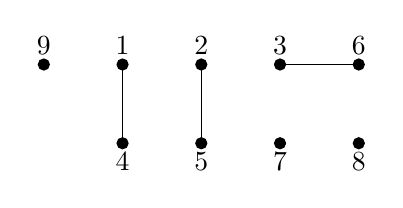
\begin{tikzpicture}
        \draw[fill=black] (0,0) circle (2pt) node[anchor=south]{9};
        \draw[fill=black] (1,0) circle (2pt) node[anchor=south]{1};
        \draw[fill=black] (2,0) circle (2pt) node[anchor=south]{2};
        \draw[fill=black] (3,0) circle (2pt) node[anchor=south]{3};
        \draw[fill=black] (4,0) circle (2pt) node[anchor=south]{6};
        \draw[fill=black] (1,-1) circle (2pt) node[anchor=north]{4};
        \draw[fill=black] (2,-1) circle (2pt) node[anchor=north]{5};
        \draw[fill=black] (3,-1) circle (2pt) node[anchor=north]{7};
        \draw[fill=black] (4,-1) circle (2pt) node[anchor=north]{8};
        
        \draw[] (1,0)--(1,-1);
        \draw[] (2,0)--(2,-1);
        \draw[] (3,0)--(4,0);
    \end{tikzpicture}
\end{center}

\begin{align*}
    \text{code: } & (\not1, \not2, \not3, \not3, 3, 2, 1) \\
    \text{vertices: } & (1, 2, 3, \not4, \not5, \not6, \not7, 8, 9)
\end{align*}
\begin{center}
    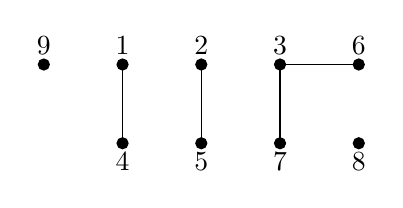
\begin{tikzpicture}
        \draw[fill=black] (0,0) circle (2pt) node[anchor=south]{9};
        \draw[fill=black] (1,0) circle (2pt) node[anchor=south]{1};
        \draw[fill=black] (2,0) circle (2pt) node[anchor=south]{2};
        \draw[fill=black] (3,0) circle (2pt) node[anchor=south]{3};
        \draw[fill=black] (4,0) circle (2pt) node[anchor=south]{6};
        \draw[fill=black] (1,-1) circle (2pt) node[anchor=north]{4};
        \draw[fill=black] (2,-1) circle (2pt) node[anchor=north]{5};
        \draw[fill=black] (3,-1) circle (2pt) node[anchor=north]{7};
        \draw[fill=black] (4,-1) circle (2pt) node[anchor=north]{8};
        
        \draw[] (1,0)--(1,-1);
        \draw[] (2,0)--(2,-1);
        \draw[] (3,0)--(4,0);
        \draw[] (3,0)--(3,-1);
    \end{tikzpicture}
\end{center}

\begin{align*}
    \text{code: } & (\not1, \not2, \not3, \not3, \not3, 2, 1) \\
    \text{vertices: } & (1, 2, 3, \not4, \not5, \not6, \not7, \not8, 9)
\end{align*}
\begin{center}
    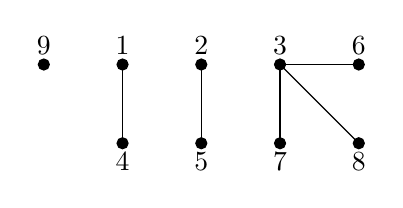
\begin{tikzpicture}
        \draw[fill=black] (0,0) circle (2pt) node[anchor=south]{9};
        \draw[fill=black] (1,0) circle (2pt) node[anchor=south]{1};
        \draw[fill=black] (2,0) circle (2pt) node[anchor=south]{2};
        \draw[fill=black] (3,0) circle (2pt) node[anchor=south]{3};
        \draw[fill=black] (4,0) circle (2pt) node[anchor=south]{6};
        \draw[fill=black] (1,-1) circle (2pt) node[anchor=north]{4};
        \draw[fill=black] (2,-1) circle (2pt) node[anchor=north]{5};
        \draw[fill=black] (3,-1) circle (2pt) node[anchor=north]{7};
        \draw[fill=black] (4,-1) circle (2pt) node[anchor=north]{8};
        
        \draw[] (1,0)--(1,-1);
        \draw[] (2,0)--(2,-1);
        \draw[] (3,0)--(4,0);
        \draw[] (3,0)--(3,-1);
        \draw[] (3,0)--(4,-1);
    \end{tikzpicture}
\end{center}

\begin{align*}
    \text{code: } & (\not1, \not2, \not3, \not3, \not3, \not2, 1) \\
    \text{vertices: } & (1, 2, \not3, \not4, \not5, \not6, \not7, \not8, 9)
\end{align*}
\begin{center}
    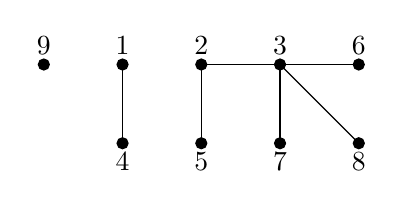
\begin{tikzpicture}
        \draw[fill=black] (0,0) circle (2pt) node[anchor=south]{9};
        \draw[fill=black] (1,0) circle (2pt) node[anchor=south]{1};
        \draw[fill=black] (2,0) circle (2pt) node[anchor=south]{2};
        \draw[fill=black] (3,0) circle (2pt) node[anchor=south]{3};
        \draw[fill=black] (4,0) circle (2pt) node[anchor=south]{6};
        \draw[fill=black] (1,-1) circle (2pt) node[anchor=north]{4};
        \draw[fill=black] (2,-1) circle (2pt) node[anchor=north]{5};
        \draw[fill=black] (3,-1) circle (2pt) node[anchor=north]{7};
        \draw[fill=black] (4,-1) circle (2pt) node[anchor=north]{8};
        
        \draw[] (1,0)--(1,-1);
        \draw[] (2,0)--(2,-1);
        \draw[] (3,0)--(4,0);
        \draw[] (3,0)--(3,-1);
        \draw[] (3,0)--(4,-1);
        \draw[] (2,0)--(3,0);
    \end{tikzpicture}
\end{center}

\begin{align*}
    \text{code: } & (\not1, \not2, \not3, \not3, \not3, \not2, \not1) \\
    \text{vertices: } & (1, \not2, \not3, \not4, \not5, \not6, \not7, \not8, 9)
\end{align*}
\begin{center}
    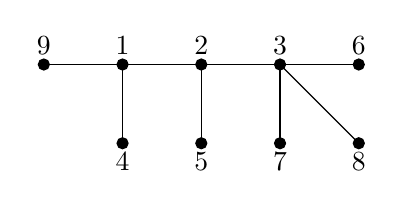
\begin{tikzpicture}
        \draw[fill=black] (0,0) circle (2pt) node[anchor=south]{9};
        \draw[fill=black] (1,0) circle (2pt) node[anchor=south]{1};
        \draw[fill=black] (2,0) circle (2pt) node[anchor=south]{2};
        \draw[fill=black] (3,0) circle (2pt) node[anchor=south]{3};
        \draw[fill=black] (4,0) circle (2pt) node[anchor=south]{6};
        \draw[fill=black] (1,-1) circle (2pt) node[anchor=north]{4};
        \draw[fill=black] (2,-1) circle (2pt) node[anchor=north]{5};
        \draw[fill=black] (3,-1) circle (2pt) node[anchor=north]{7};
        \draw[fill=black] (4,-1) circle (2pt) node[anchor=north]{8};
        
        \draw[] (1,0)--(1,-1);
        \draw[] (2,0)--(2,-1);
        \draw[] (3,0)--(4,0);
        \draw[] (3,0)--(3,-1);
        \draw[] (3,0)--(4,-1);
        \draw[] (2,0)--(3,0);
        \draw[] (1,0)--(2,0);
        \draw[] (0,0)--(1,0);
    \end{tikzpicture}
\end{center}

\end{multicols}


\exercise{9}{
    Let $G$ be a connected graph with $n$ vertices. Define the tree graph $T(G)$ to be the graph with vertices labeled by the spanning trees of $G$ $T_1, T_2, \dots , T_{T(G)}$, with $T_i$ and $T_j$ adjacent if they have $n - 2$ edges in common. Show that $T(G)$ is connected.
}

Suppose $T(G)$ is not connected, so there are at least two vertices such that there does not exist a walk in $T(G)$ between them. Consider the set of all pairs of vertices in $T(G)$ for which no walk exists between them (disconnected). Each of these pairs of vertices (trees) share some integer number of edges from 0 to $n-1$. We select $T_a$ and $T_b$ to be the pair of disconnected vertices which share the greatest number of edges. 

Since $T_a$ and $T_b$ are not the same tree, there must be some edge $e_1$ such that $e_1\in V(T_b)$ but $e_1\notin V(T_a)$. We now consider the graph $T_a+e_1$. Adding $e_1$ has created a graph with $n$ edges, and therefore a cycle. There must be some $e_2$ in this cycle which is not in $T_b$, since $T_b$ is a tree. So we consider the graph $T_c = T_a + e_1 - e_2$, which is a tree, since deleting $e_2$ has removed the one cycle.

Since from $T_a$ to $T_C$, we added $e_1\in T_b$ and deleted $e_2\notin T_b$, we know that $T_c$ shares one more edge with $T_b$ than $T_a$. As well, $T_a$ and $T_c$ share $n-2$ edges, since $T_c$ has all $n-1$ edges in $T_a$ except $e_2$, so $T_a$ and $T_c$ are connected in $T(G)$.

Since $T_a$ and $T_b$ are disconnected, $T_c$ and $T_b$ must also be disconnected. However, $T_c$ and $T_b$ share one more edge than $T_a$ and $T_b$, which we supposed to be the pair of disconnected vertices in $T(G)$ which share the greatest number of edges. This is a contradiction, so our assumption that $T(G)$ is not connected must be false. Therefore, $T(G)$ is connected.







\end{document}